\subsubsection{V2I}
% 
Vehicle-to-Infrastructure technologies are still under development, but it has great potential. Its main idea is communication with vehicle by any road side unit (e.g. traffic lights, road sensors) to prevent accidents and improve road efficiency.\par
% 
% Vehicle-to-Infrastructure Technologies Expected to offer Benefits
\begin{figure}[h]
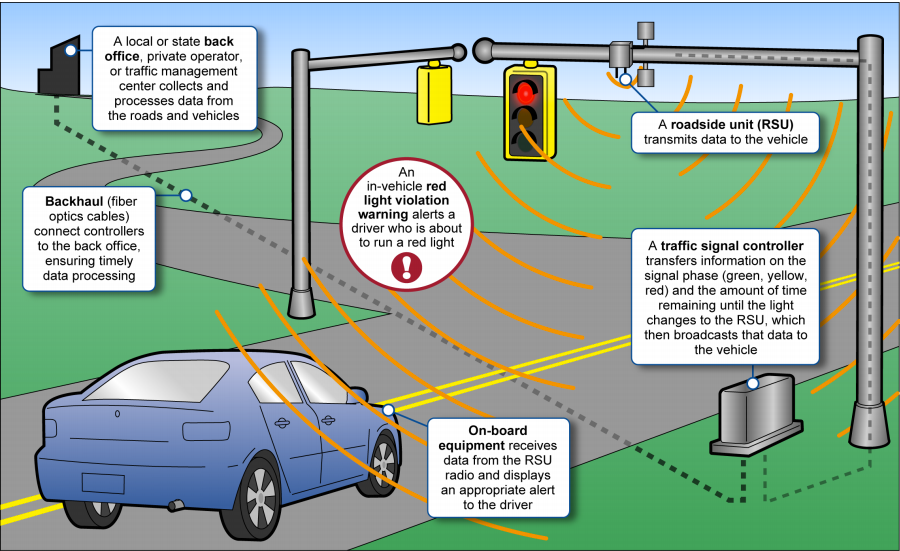
\includegraphics[width=\textwidth]{V2I}
\caption{V21 implementation. Taken from \cite{U.S.GovernmentAccountabilityOffice2015IntelligentExist}.}
\label{fig:V2Iimplementation}
\centering
\end{figure}
% 
There no standards yet of what V2I system architecture should consist of. Architecture framework defined by USDOTs' ITS Joint Program Office \cite{Dr.Gaspar2014HighlySystems} states, that minimal parts for V2I system are:
\begin{itemize}
    \item Vehicle On-Board Unit
    \item Roadside Unit
    \item Safe Communication Channel.
\end{itemize}
% 
Communication is based on 802.11 standard by IEEE, which will be discussed in detail in following chapters. A frequency spectrum in 5.9 GHz range was allocated for exact means in U.S. and Europe \cite{2011TheTechnology}. Although, there are some concerns sharing allocated spectrum, since Middle Class Tax Relief and Job Creation Act of 2012 allowed use of 5.9GHz spectrum for any unlicensed devices and that could cause harmful interference for sending and receiving data in V2I communication \cite{U.S.GovernmentAccountabilityOffice2015IntelligentExist}.\par
% 
Despite any concerns, Vehicle-to-Infrastructure is quickly developing and gaining a lot of attention from scientists and businessman worldwide.\par
%
//To be restructured.
% 
\begin{figure}[h]
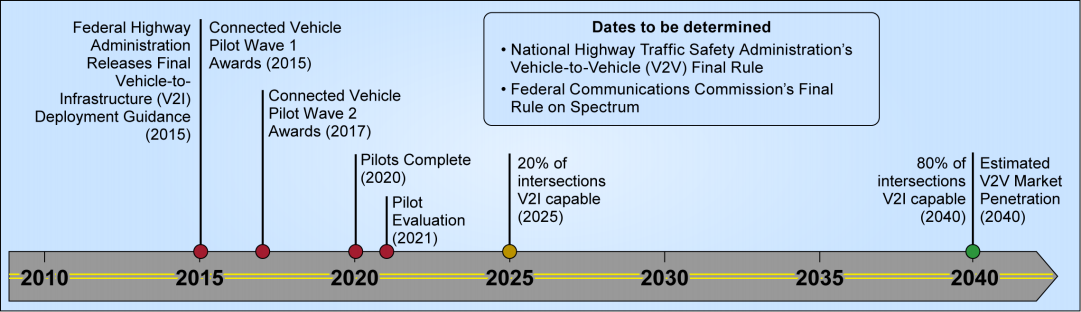
\includegraphics[width=\textwidth]{V2Xtimeline}
\caption{V21 development path. Taken from \cite{U.S.GovernmentAccountabilityOffice2015IntelligentExist}.}
\label{fig:V2Idevelopment}
\centering
\end{figure}
